\documentclass[english, aspectratio=169]{beamer}
% english is for the language used in standard texts (figures, tables etc)
% aspectratio of 16:9 or set it for more old school to 4:3 (without the ':')

% ---------------------------------------------------------------------------- %
% Load base preamble
% ---------------------------------------------------------------------------- %
\usepackage{import}
\subimport{./preamble/}{beamer.tex}

\metroset{sectionpage=none}

% ---------------------------------------------------------------------------- %
% Local settings
% ---------------------------------------------------------------------------- %
% https://tex.stackexchange.com/a/20613
\newcommand\hcancel[2][black]{\setbox0=\hbox{$#2$}%
  \rlap{\raisebox{.35\ht0}{\textcolor{#1}{\rule{\wd0}{1pt}}}}#2}

\newcommand{\B}[0]{\ensuremath{\mathbb{B}}}

\newcommand{\sort}[0]{\text{sort}}

\newcommand{\triple}[3]{\ensuremath{(#1, #2, #3)}}
\renewcommand{\arc}[3]{\ensuremath{#1 \xrightarrow{_{#2}} #3}}

\tikzstyle{plot_adiar_old}=[color=black, dashed, mark=none, line width=0.5pt]
\tikzstyle{plot_adiar}=[color=black, mark=o, mark size=1pt, line width=1pt]
\tikzstyle{plot_buddy}=[color=red, mark=o, mark size=1pt, line width=0.7pt]
\tikzstyle{plot_cudd}=[color=blue, mark=diamond, mark size=1pt, line width=0.7pt]
\tikzstyle{plot_sylvan}=[color=purple, mark=square, mark size=1pt, line width=0.7pt]

% Horizontal legends: https://tex.stackexchange.com/a/101578
% argument #1: any options
\makeatletter
\newenvironment{customlegend}[1][]{%
    \begingroup
    % inits/clears the lists (which might be populated from previous
    % axes):
    \pgfplots@init@cleared@structures
    \pgfplotsset{#1}%
}{%
    % draws the legend:
    \pgfplots@createlegend
    \endgroup
}%

% makes \addlegendimage available (typically only available within an
% axis environment):
\def\addlegendimage{\pgfplots@addlegendimage}
\makeatother

% ------------------------------------------------------------------------------
% TITLEPAGE
% ------------------------------------------------------------------------------
\title{
  Predicting Memory Demands of BDD Operations\\using Maximum Graph Cuts
}

\author{{\bf Steffan Christ S{\o}lvsten} and Jaco van de Pol}

\institute{
\includegraphics[width=0.2\linewidth]{external/aulogo_uk_var2_black.eps}}

\date{ATVA 2023}

\begin{document}

\titleframe

\begin{frame}
  \begin{figure}
    \centering

    \only<1-2> {
      \hspace{0.385\linewidth} %
      %
      \begin{tikzpicture}
        \begin{axis}[%
          width=0.515\linewidth, height=0.42\linewidth,
          every tick label/.append style={font=\scriptsize},
          % x-axis
          xlabel={Problem Complexity (\# BDD nodes)},
          xmajorgrids=true,
          xmin=40000000,
          xmax=300000000000,
          xmode = log,
          % y-axis
          ymin=0.001,
          ymax=1000000,
          ymode=log,
          ytick={0.001,0.01,0.1,1,10,100,1000,10000,100000,1000000},
          ylabel={Time (s)},
          yminorgrids=false,
          ymajorgrids=true,
          grid style={dashed,black!20},
          ]

          \addplot+ [style=plot_buddy]
          table {./data/queens_buddy_time.tex};

          \addplot+ [style=plot_cudd]
          table {./data/queens_cudd_time.tex};

          \addplot+ [style=plot_sylvan]
          table {./data/queens_sylvan_time.tex};

          \only<2-> {
            \addplot+ [style=plot_adiar]
            table {./data/queens_adiar_time.v1.0.0.tex};
          }
        \end{axis}
      \end{tikzpicture}
    }
    \only<3-> {
      \begin{tikzpicture}
        \begin{axis}[%
          width=0.88\linewidth, height=0.42\linewidth,
          every tick label/.append style={font=\scriptsize},
          % x-axis
          xlabel={Problem Complexity (\# BDD nodes)},
          xmajorgrids=true,
          xmin=12000,
          xmax=300000000000,
          xmode = log,
          % y-axis
          ymin=0.001,
          ymax=1000000,
          ymode=log,
          ytick={0.001,0.01,0.1,1,10,100,1000,10000,100000,1000000},
          ylabel={Time (s)},
          yminorgrids=false,
          ymajorgrids=true,
          grid style={dashed,black!20},
          ]

          \addplot+ [style=plot_buddy]
          table {./data/queens_buddy_time.tex};

          \addplot+ [style=plot_cudd]
          table {./data/queens_cudd_time.tex};

          \addplot+ [style=plot_sylvan]
          table {./data/queens_sylvan_time.tex};

          \only<3>{
            \addplot+ [style=plot_adiar]
            table {./data/queens_adiar_time.v1.0.0.tex};
          }
         \only<4>{
           \addplot+ [style=plot_adiar_old]
           table {./data/queens_adiar_time.v1.0.0.tex};

           \addplot+ [style=plot_adiar]
           table {./data/queens_adiar_time.v1.2.0.tex};
         }
        \end{axis}
      \end{tikzpicture}
    }

    \begin{tikzpicture}
      \only<-3>{
        \begin{customlegend}[
          legend columns=-1,
          legend style={draw=none,column sep=1ex},
          legend entries={BuDDy, CUDD, Sylvan, Adiar v1.0}
          ]
          \addlegendimage{style=plot_buddy}
          \addlegendimage{style=plot_cudd}
          \addlegendimage{style=plot_sylvan}
          \addlegendimage{style=plot_adiar}
        \end{customlegend}
      }
      \only<4>{
        \begin{customlegend}[
          legend columns=-1,
          legend style={draw=none,column sep=1ex},
          legend entries={BuDDy, CUDD, Sylvan, Adiar v1.2}
          ]
          \addlegendimage{style=plot_buddy}
          \addlegendimage{style=plot_cudd}
          \addlegendimage{style=plot_sylvan}
          \addlegendimage{style=plot_adiar}
        \end{customlegend}
      }
    \end{tikzpicture}

    \caption{Running Time to solve $N$-\emph{Queens} problems.}
  \end{figure}
\end{frame}

\begin{frame}
  \begin{center}
  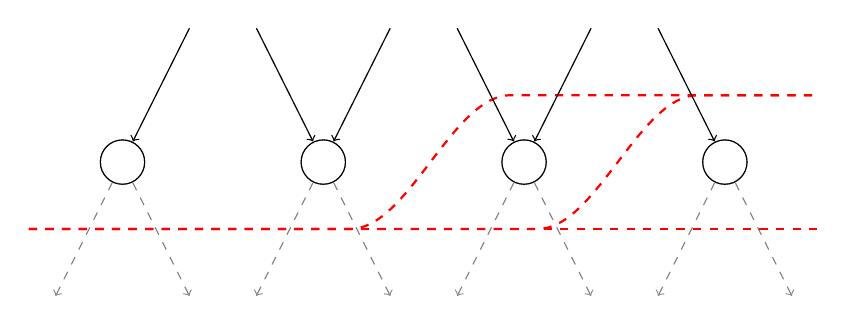
\begin{tikzpicture}[scale=1.7, every node/.style={transform shape}]
    % cut coordinates
    \coordinate (cut_start) at (-0.7,-0.5);
    \coordinate (cut_end_low) at (5.2,-0.5);
    \path (cut_end_low) +(0,1) coordinate (cut_end_high);

    % --------------------------------------------------------------------------
    % before
    \onslide<1> {
      \node[shape = circle, draw = gray] at (0,0)  (0_before) {};
      \draw[gray, dashed, <-] (0_before) -- ++(0.5,1.0);
    }

    % after
    \onslide<2-> {
      \node[shape = circle, draw = black] at (0,0) (0_after) {};
      \draw[black, <-] (0_after) -- ++(0.5,1.0);

      \draw[gray, dashed, ->] (0_after) -- ++(-0.5,-1);
      \draw[gray, dashed, ->] (0_after) -- ++(0.5,-1);
    }

    % --------------------------------------------------------------------------
    % before
    \onslide<-2> {     
      \node[shape = circle, draw = gray] at (1.5,0) (1_before) {};
      \draw[gray, dashed, <-] (1_before) -- ++(-0.5,1.0);
      \draw[gray, dashed, <-] (1_before) -- ++(0.5, 1.0);
    }

    % after
    \onslide<3-> {
      \node[shape = circle, draw = black] at (1.5,0) (1_after) {};
      \draw[black, <-] (1_after) -- ++(-0.5,1.0);
      \draw[black, <-] (1_after) -- ++(0.5, 1.0);

      \draw[gray, dashed, ->] (1_after) -- ++(-0.5,-1);
      \draw[gray, dashed, ->] (1_after) -- ++(0.5,-1);
    }

    % cut
    \onslide<4> {
      \draw[thick, dashed, red]
        (cut_start) -- ++(2.4,0.0) cos ++(0.6,0.5) sin ++(0.6,0.5) -- (cut_end_high)
      ;
    }
    
    % --------------------------------------------------------------------------
    % before
    \onslide<-4> {
      \node[shape = circle, draw = gray] at (3.0,0) (2_before) {};
      \draw[gray, dashed, <-] (2_before) -- ++(-0.5,1.0);
      \draw[gray, dashed, <-] (2_before) -- ++(0.5,1.0);
    }

    % after    
    \onslide<5-> {
      \node[shape = circle, draw = black] at (3.0,0) (2_after) {};
      \draw[black, <-] (2_after) -- ++(-0.5, 1.0);
      \draw[black, <-] (2_after) -- ++(0.5, 1.0);

      \draw[gray, dashed, ->] (2_after) -- ++(-0.5,-1);
      \draw[gray, dashed, ->] (2_after) -- ++(0.5,-1);
    }

    % cut
    \onslide<5> {
      \draw[thick, dashed, red]
        (cut_start) -- ++(3.8,0.0) cos ++(0.6,0.5) sin ++(0.6,0.5) -- (cut_end_high)
      ;
    }

    % --------------------------------------------------------------------------
    % before
    \onslide<-5> {
      \node[shape = circle, draw = gray] at (4.5,0) (3_before) {};
      \draw[gray, dashed, <-] (3_before) -- ++(-0.5,1.0);
    }

    % after
    \onslide<6-> {
      \node[shape = circle, draw = black] at (4.5,0) (3_after) {};
      \draw[black, <-] (3_after) -- ++(-0.5,1.0);      

      \draw[gray, dashed, ->] (3_after) -- ++(-0.5,-1);
      \draw[gray, dashed, ->] (3_after) -- ++(0.5,-1);
    }

    % cut
    \onslide<6> {
      \draw[thick, dashed, red]
        (cut_start) -- (cut_end_low)
      ;
    }
  \end{tikzpicture}
\end{center}
\end{frame}

\begin{frame}
  \begin{center}
    \textbf{\LARGE \emph{i}-level cut}
  \end{center}
  \begin{columns}
    \begin{column}{0.55\textwidth}
      \begin{tikzpicture}[scale=0.9]
        % levels
\node (Lcal) {\color{gray} $\mathcal{L}$};

\node[below=0.5cm of Lcal] (Lj) {\color{gray} $j$};
\node[below=0.5cm of Lj] (Lj1) {\color{gray} $j+1$};
\node[below=0.5cm of Lj1] (Ldots) {\color{gray} $\vdots$};
\node[below=0.6cm of Ldots] (Lji) {\color{gray} $j+i$};

\draw[dashed, gray]
  ($ (Lj) + (1,0) $) edge ($ (Lj) + (7,0) $)
;

\draw[dashed, gray]
  ($ (Lji) + (1,0) $) edge ($ (Lji) + (7,0) $)
;

% nodes
\node[shape = circle, draw = black, fill=white, right=2cm of Lj] (j_1) {};
\node[shape = circle, draw = black, fill=white, right=3cm of Lj] (j_2) {};
\node[shape = circle, draw = black, fill=white, right=5cm of Lj] (j_3) {};

\node[shape = circle, draw = black, fill=white, right=2.5cm of Lj1] (j1_1) {};
\node[shape = circle, draw = black, fill=white, right=4cm of Lj1] (j1_2) {};

\node[right=3.8cm of Ldots] (jdot_1) {$\cdot$};
\node[right=5.3cm of Ldots] (jdot_2) {$\cdot$};

\node[shape = circle, draw = black, fill=white, right=1.5cm of Lji] (ji_1) {};
\node[shape = circle, draw = black, fill=white, right=3cm of Lji] (ji_2) {};
\node[shape = circle, draw = black, fill=white, right=5cm of Lji] (ji_3) {};

% arcs
\draw[->]
% to level j
  ($ (j_1) + (-0.5,0.5) $) edge (j_1)
  ($ (j_1) + (0.5,0.5) $) edge (j_1)

  ($ (j_2) + (0,0.5) $) edge (j_2)

  ($ (j_3) + (-0.5,0.5) $) edge (j_3)
  ($ (j_3) + (0.5,0.5) $) edge (j_3)

% to level j+1
  (j_1) edge (j1_1)
  (j_2) edge (j1_1)
  ($ (j_2) + (1,0.5) $) edge (j1_2)
  (j_3) edge (j1_2)

% to levels in between
  (j1_2) edge[bend right=10] (jdot_1)
  (j1_2) edge[bend left=20] (jdot_2)
  (j_3) edge[bend left=15] (jdot_2)
  (j_3) edge[bend left=50] (jdot_2)

% to level j+i
  ($ (j_1) + (-0.7,0.5) $) edge[bend right=10] (ji_1)
  (j_1) edge[bend left=5] (ji_1)
  (j_2) edge[bend left=5] (ji_2)
  (jdot_1) edge[bend left=10] (ji_2)
  (jdot_2) edge[bend left=20] (ji_3)
  (jdot_2) edge[bend right=20] (ji_3)

% past level j+i
  (j1_1) edge[bend left=5] ($ (ji_1) + (0.7,-0.5) $)
  (jdot_1) edge[bend right=10] ($ (ji_2) + (1,-0.5) $)
  (ji_1) edge ($ (ji_1) + (-0.5,-0.5) $)
  (ji_1) edge ($ (ji_1) + (0.5,-0.5) $)
  (ji_2) edge ($ (ji_2) + (0,-0.5) $)
  (ji_3) edge ($ (ji_3) + (-0.5,-0.5) $)
  ($ (j_3) + (1,0.5) $) -> ($ (ji_3) + (1,-0.5) $)
;

% cut
\draw[thick, dashed, red]
  ($ (j_1) + (-1.2, -1.5) $) sin
  ($ (j_2) + (-0.2, -0.5) $) cos
  ($ (j_2) + (0.4, -2) $) sin
  ($ (jdot_1) + (0.0, -0.5) $) cos
  ($ (jdot_1) + (0.2, 0) $) --
  ($ (j1_2) + (-0.3, 0) $) sin
  ($ (j1_2) + (0, 0.5) $) cos
  ($ (j1_2) + (0.4, 0) $) sin
  ($ (j1_2) + (1.1, -1.8) $) --
  ($ (j1_2) + (2.2, -1.8) $)
;

      \end{tikzpicture}
    \end{column}
    \begin{column}{0.44\textwidth}
      \onslide<2-> {
        \begin{lemma}[\footnotesize S{\o}lvsten, Van de Pol 2023]
          The maximum $i$-level cut problem is in P for $i \in \{ 1,2 \}$.
        \end{lemma}

        \begin{theorem}[\footnotesize Lampis, Kaouri, Mitsou 2011]
          The maximum $i$-level cut problem is NP-complete for $i \geq 4$.
        \end{theorem}
      }
    \end{column}
  \end{columns}
\end{frame}

\blankframe

\begin{frame}
  \begin{theorem}[\footnotesize S{\o}lvsten, Van de Pol 2023]
    Given maximum $2$-level cuts size $C_f$ for $f$ and $C_g$ for $g$, the
    maximum $2$-level cut for $f \odot g$ is less than or equal to
    $C_f \cdot C_g$.
  \end{theorem}

  \begin{proof}
    % Every edge in the output corresponds to pairs of edges in the input. Any
    % edge not part of the input's maximum cut can be charged to one that is.

    \only<1>{
      \vspace{1pt} % HACK: compensate for difference in height of figure
      \begin{center}
        \begin{tikzpicture}[baseline=(a1.base)]
          % nodes of level j
\node[shape = circle, draw = black] (a1) {$a_1$};
\node[shape = circle, draw = black, right=of a1] (a2) {$a_2$};

% subtrees of levels > j
\node[shape = rectangle, draw = black, below left=0.5cm and .35cm of a1] (top) {$\top$};
\node[below right=0.5cm and .35cm of a1] (alpha1) {$\alpha_1$};
\node[below right=0.5cm and .35cm of a2] (alpha2) {$\alpha_2$};
\node[below right=0.5cm and 2.0cm of a2] (alpha3) {$\alpha_3$};

% arcs in the max-cut
\draw[->]
($ (a1) + (-0.2, 1) $) edge (a1)
($ (a1) + (0.2, 1) $)  edge (a1)
(a1)                   edge (alpha1)
(a1)                   edge (top)
($ (a2) + (0, 1) $)    edge (a2)
(a2)                   edge (alpha1)
(a2)                   edge (alpha2)
($ (a2) + (2.2, 1) $)  edge (alpha3)
($ (a2) + (2.9, 1) $)   ->  (alpha3)
;

% cut line
\draw[thick, dashed, red]
($ (a1) - (0.9, 0.5) $) edge ($ (alpha3) + (0.6, 0.5) $)
;

        \end{tikzpicture}
        \qquad
        $\odot$
        \qquad
        \begin{tikzpicture}[baseline=(b1.base)]
          % nodes of level j
\node[shape = circle, draw = black] (b1) {$b_1$};

% subtrees of levels > j
\node[below left=0.5cm and .35cm of a1]  (beta1) {$\beta_1$};
\node[shape = rectangle, draw = black, below right=0.5cm and .35cm of a1] (bot) {$\bot$};

% arcs in the max-cut
\draw[->]
($ (b1) + (-0.4, 1) $) edge (b1)
($ (b1) + (0, 1) $)    edge (b1)
($ (b1) + (0.4, 1) $)  edge (b1)
(b1) edge (beta1)
(b1) edge (bot)
($ (bot) + (0, 2) $)    ->  (bot)
;

% cut line
\draw[thick, dashed, red]
($ (b1) + (-0.8, 0.8) $) edge ($ (b1) + (1.3, 0.8) $)
;

        \end{tikzpicture}
      \end{center}
      \vspace{2pt} % HACK: compensate for difference in height of figures
    }
    \only<2>{
      \begin{center}
        \begin{tikzpicture}[baseline=(a1_b1__1.base)]
          % nodes
\node[shape = circle, draw = black]                    (a1_b1)     {\tiny $a_1, b_1$};
\node[below left=0.6cm and -0.3cm of a1_b1] (a1_b1__1) {\tiny $\top, \beta_1$};
\node[below right=0.6cm and -0.3cm of a1_b1] (a1_b1__2) {\tiny $\alpha_1, \bot$};

\node[shape = circle, draw = black, right=of a1_b1]    (a1_bot)  {\tiny $a_1, \bot$};
\node[below left=0.6cm and -0.3cm of a1_bot] (a1_bot__1) {\tiny $\top, \bot$};
\node[below right=0.6cm and -0.3cm of a1_bot] (a1_bot__2) {\tiny $\alpha_1, \bot$};

\node[shape = circle, draw = black, right=of a1_bot] (a2_b1)     {\tiny $a_2, b_1$};
\node[below left=0.6cm and -0.3cm of a2_b1]  (a2_b1__1) {\tiny $\alpha_1, \beta_1$};
\node[below right=0.6cm and -0.3cm of a2_b1] (a2_b1__2) {\tiny $\alpha_1, \bot$};

\node[shape = circle, draw = black, right=of a2_b1]    (a2_bot)  {\tiny $a_2, \bot$};
\node[below left=0.6cm and -0.3cm of a2_bot]  (a2_bot__1) {\tiny $\alpha_1, \bot$};
\node[below right=0.6cm and -0.3cm of a2_bot] (a2_bot__2) {\tiny $\alpha_2, \bot$};

\node[shape = circle, draw = black, right=of a2_bot] (alpha3_b1) {\tiny $\alpha_3, b_1$};
\node[below left=0.6cm and -0.3cm of alpha3_b1]  (alpha3_b1__1) {\tiny $\alpha_3, \beta_1$};
\node[below right=0.6cm and -0.3cm of alpha3_b1] (alpha3_b1__2) {\tiny $\alpha_3, \bot$};

\node[below right=0.6cm and 1cm of alpha3_b1] (alpha3_bot) {\tiny $\alpha_3, \bot$};

% arcs in the max-cut
\draw[->]
($ (a1_b1) + (-1, 1) $)           edge (a1_b1)
($ (a1_b1) + (-0.6, 1) $)         edge (a1_b1)
($ (a1_b1) + (-0.2, 1) $)         edge (a1_b1)
($ (a1_b1) + (0.2, 1) $)          edge (a1_b1)
($ (a1_b1) + (0.6, 1) $)          edge (a1_b1)
($ (a1_b1) + (1, 1) $)            edge (a1_b1)
(a1_b1)                           edge (a1_b1__1)
(a1_b1)                           edge (a1_b1__2)
($ (a1_bot) + (0, 1) $)           edge (a1_bot)
(a1_bot)                          edge (a1_bot__1)
(a1_bot)                          edge (a1_bot__2)
($ (a2_b1) + (-0.4, 1) $)         edge (a2_b1)
($ (a2_b1) + (0, 1) $)            edge (a2_b1)
($ (a2_b1) + (0.4, 1) $)          edge (a2_b1)
(a2_b1)                           edge (a2_b1__1)
(a2_b1)                           edge (a2_b1__2)
($ (a2_bot) + (0, 1) $)           edge (a2_bot)
(a2_bot)                          edge (a2_bot__1)
(a2_bot)                          edge (a2_bot__2)
($ (alpha3_b1) + (-1, 1) $)       edge (alpha3_b1)
($ (alpha3_b1) + (-0.6, 1) $)     edge (alpha3_b1)
($ (alpha3_b1) + (-0.2, 1) $)     edge (alpha3_b1)
($ (alpha3_b1) + (0.2, 1) $)      edge (alpha3_b1)
($ (alpha3_b1) + (0.6, 1) $)      edge (alpha3_b1)
($ (alpha3_b1) + (1, 1) $)        edge (alpha3_b1)
(alpha3_b1)                       edge (alpha3_b1__1)
(alpha3_b1)                       edge (alpha3_b1__2)
($ (alpha3_bot) + (-0.3, 2.15) $) edge (alpha3_bot)
($ (alpha3_bot) + (0.4, 2.15) $)   -> (alpha3_bot)
;

% % cut line
\draw[thick, dashed, red]
($ (a1_b1) + (-1.0, 0.9) $) --
($ (a1_b1) + (0.0, 0.9) $) cos
($ (a1_b1) + (1, 0) $) sin
($ (a1_bot) + (0, -0.7) $) cos
($ (a1_bot) + (1, 0) $) sin
($ (a2_b1) + (0, 0.9) $) cos
($ (a2_b1) + (1, 0) $) sin
($ (a2_bot) + (0, -0.7) $) cos
($ (a2_bot) + (1, 0) $) sin
($ (alpha3_b1) + (0, 0.9) $) cos
($ (alpha3_b1) + (1, 0.4) $) sin
($ (alpha3_b1) + (2.2, 0) $)
;

        \end{tikzpicture}
      \end{center}
    }
    \vspace{2pt} % HACK: make it the same height as the next slide
  \end{proof}
\end{frame}

\begin{frame}
  \begin{lemma}[\footnotesize S{\o}lvsten, Van de Pol 2023]
    The maximum $2$-level cut for $f$ is at most $\tfrac{3}{2}$ larger
    than its maximum $1$-level cut.
  \end{lemma}
  \vspace{14pt}
  \begin{proof}
    % The maximum $1$-level cut bounds the number of available in-going and
    % out-going edges. Hence, it bounds the number of nodes that can be moved to
    % increase the cut size.

    \begin{center}
      \begin{tikzpicture}
  % nodes of level j
  \node[shape = circle, draw = black] (a1) {$a_1$};
  \node[shape = circle, draw = black, right=of a1] (a2) {$a_2$};
  \node[shape = circle, draw = black, right=of a2] (a3) {$a_3$};

  % subtrees of levels > j
  \node[shape = rectangle, draw = black, below left=0.5cm and .35cm of a1] (top) {$\top$};
  \node[below right=0.5cm and .35cm of a1] (alpha1) {$\alpha_1$};
  \node[below right=0.5cm and .35cm of a2] (alpha2) {$\alpha_2$};
  \node[below right=0.5cm and .35cm of a3] (alpha3) {$\alpha_3$};
  \node[below right=0.5cm and 2.0cm of a3] (alpha4) {$\alpha_4$};

  % arcs in the max-cut
  \draw[->]
  ($ (a1) + (-0.2, 1) $) edge (a1)
  ($ (a1) + (0.2, 1) $)  edge (a1)
  (a1)                   edge (alpha1)
  (a1)                   edge (top)
  ($ (a2) + (0, 1) $)    edge (a2)
  (a2)                   edge (alpha1)
  (a2)                   edge (alpha2)
  ($ (a3) + (0, 1) $)    edge (a3)
  (a3)                   edge (alpha2)
  (a3)                   edge (alpha3)
  ($ (a3) + (2.2, 1) $)  edge (alpha4)
  ($ (a3) + (2.9, 1) $)   ->  (alpha4)
  ;

  % cut line
  \onslide<1>{
    \draw[thick, dashed, red]
    ($ (a1) + (-0.9, 0.7) $) -- ($ (alpha4) + (0.6, 1.7) $)
    ;
  }
  \onslide<2>{
    \draw[thick, dashed, red]
    ($ (a1) + (-0.9, 0.7) $) --
    ($ (a1) + (0.5, 0.7) $) cos
    ($ (a2) + (-0.7, 0)$) sin
    ($ (a2) + (0, -0.7)$) cos
    ($ (a2) + (0.7, 0)$) sin
    ($ (a2) + (1.4, 0.7)$) --
    ($ (alpha4) + (0.6, 1.7) $)
    ;
  }
  \onslide<3>{
    \draw[thick, dashed, red]
    ($ (a1) + (-0.9, 0.7) $) --
    ($ (a1) + (0.5, 0.7) $) cos
    ($ (a2) + (-0.7, 0)$) sin
    ($ (a2) + (0, -0.7)$) --
    ($ (a3) + (0, -0.7)$) cos
    ($ (a3) + (0.7, 0)$) sin
    ($ (a3) + (1.4, 0.7)$) --
    ($ (alpha4) + (0.6, 1.7) $)
    ;
  }
\end{tikzpicture}
    \end{center}
  \end{proof}
\end{frame}

\blankframe

\begin{frame}
  \begin{table}[ht!]
    \centering

    { \LARGE
      \begin{tabular}{lccc}
                    &               & +\faIcon{stopwatch}  & \faIcon{ruler}
        \\
                    &               & \normalsize Overhead & \normalsize Precision
        \\ \hline
        1-level cut & \quad : \quad & $1.0\%$  & 69.2\%
        \\
        2-level cut & \quad : \quad & $3.3\%$  & 86.3\%
      \end{tabular}
    }
  \end{table}
\end{frame}

\blankframe

\begin{frame}
  \begin{center}
    \textbf{Possible to process a}

    \vspace{8pt}

    \textbf{\Huge 1.1~GiB BDD}

    \vspace{2pt}

    \textbf{with only}

    \vspace{5pt}

    \textbf{\Large 128~MiB Memory}
  \end{center}
\end{frame}

\begin{frame}
  \vspace{20pt}

  \begin{table}[ht!]
    \centering

    { \LARGE
      \begin{tabular}{lcrl}
                     &               & \multicolumn{1}{c}{\faIcon{stopwatch}} &
        \\
                     &               & \multicolumn{1}{c}{\normalsize Running Time} &
        \\ \hline
        Adiar v1.0   & \quad : \quad & $56.5$ hours &
        \\ \onslide<2>{%
          Adiar v1.2 & \quad : \quad & \phantom{5}$4.0$ hours & \large ($-93\%$)$^1$ }
      \end{tabular}
    }
    \caption{Verification of the $15$ smallest EPFL circuits.}
  \end{table}

  \vspace{20pt}

  \onslide<2->{
    {\hrule width0.45\linewidth}

    $^1$\quad $52.1$ of these hours were saved on just verifying the
    \texttt{sin} circuit alone. }
\end{frame}

\blankframe

\begin{frame}[plain,noframenumbering]
  {\Large \textbf{Steffan Christ Sølvsten}}
  \vspace{1pt} {\hrule width0.45\linewidth}

  \vspace{5pt}

  \begin{itemize}
  \item[\faIcon{envelope}] \mailto{soelvsten@cs.au.dk}
  \item[\faIcon{twitter}] \href{https://www.twitter.com/ssoelvsten}{@ssoelvsten}
  \end{itemize}

  \vspace{10pt}

  {\Large \textbf{Adiar}}
  \vspace{1pt} {\hrule width0.45\linewidth}

  \vspace{5pt}

  \begin{itemize}
  \item[\faIcon{code}]
    \href{http://github.com/ssoelvsten/adiar}{github.com/ssoelvsten/adiar}
  \item[\faIcon{book}\hspace{2pt}]
    \href{http://ssoelvsten.github.io/adiar}{ssoelvsten.github.io/adiar}
  \end{itemize}


  \vspace{10pt}

  
\includegraphics[width=0.2\linewidth]{external/aulogo_uk_var2_black.eps}
\end{frame}

% ------------------------------------------------------------------------------ %
% Appendix
% ------------------------------------------------------------------------------ %
\begin{frame}
  \begin{figure}
    \centering

    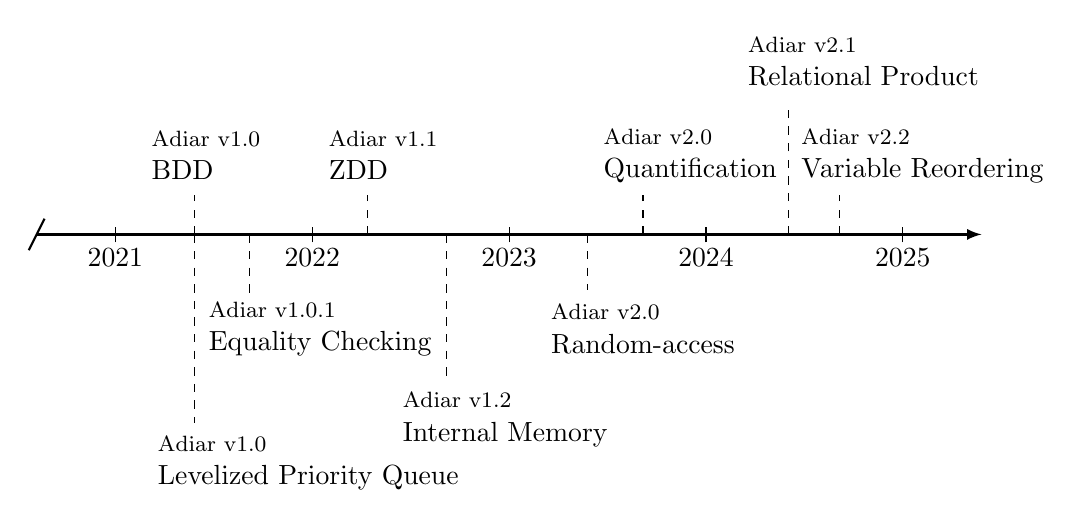
\begin{tikzpicture}
      % Primary line
\draw[-latex, thick] (0,0) -- (12,0);
\draw[thick] (0.1,0.2) -- (-0.1,-0.2);

% 2021
\draw (1,-0.1) -- ++(0,0.2);
\node at (1,-0.3) {$2021$};

\draw[dashed, color=black] (2,0) -- ++(0,0.5);
\node[color=black, align=left] at (2.15,1.0)
{\footnotesize Adiar v1.0\\BDD};

\draw[dashed, color=black] (2,0) -- ++(0,-2.4);
\node[color=black, align=left] at (3.45,-2.9)
{\footnotesize Adiar v1.0\\Levelized Priority Queue};

\draw[dashed, color=black] (2.7,0) -- ++(0,-0.8);
\node[color=black, align=left] at (3.6,-1.2)
{\footnotesize Adiar v1.0.1\\Equality Checking};

% 2022
\draw (3.5,-0.1) -- ++(0,0.2);
\node at (3.5,-0.3) {$2022$};

\draw[dashed, color=black] (4.2,0) -- ++(0,0.5);
\node[color=black, align=left] at (4.4,1.0)
{\footnotesize Adiar v1.1\\ZDD};

\draw[dashed, color=black] (5.2,0) -- ++(0,-1.8);
\node[color=black, align=left] at (5.95,-2.35)
{\footnotesize Adiar v1.2\\Internal Memory};

% 2023
\draw (6,-0.1) -- ++(0,0.2);
\node at (6,-0.3) {$2023$};

\draw[dashed, color=black] (7,0) -- ++(0,-0.7);
\node[color=black, align=left] at (7.7,-1.2)
{\footnotesize Adiar v2.0\\Random-access};

\draw[dashed, color=black] (7.7,0) -- ++(0,0.5);
\node[color=black, align=left] at (8.3,1.0)
{\footnotesize Adiar v2.0\\Quantification};

% 2024
\draw (8.5,-0.1) -- ++(0,0.2);
\node at (8.5,-0.3) (y2024) {$2024$};

\draw[dashed, color=black] (9.55,0) -- ++(0,1.6);
\node[color=black, align=left] at (10.5,2.2)
{\footnotesize Adiar v2.1\\Relational Product};

\draw[dashed, color=black] (10.2,0) -- ++(0,0.5);
\node[color=black, align=left] at (11.25,1.0)
{\footnotesize Adiar v2.2\\Variable Reordering};

% 2025
\draw (11,-0.1) -- ++(0,0.2);
\node at (11,-0.3) (y2025) {$2025$};
    \end{tikzpicture}
  \end{figure}
\end{frame}


\begin{frame}
  \begin{table}[ht!]
    \centering

    { %\footnotesize
      \begin{tabular}{r||c||cccc}
            & \faIcon{tasks}    & +\faIcon{stopwatch} & \faIcon{memory}              & \faIcon{database} & \faIcon{sync}
        \\
            & \tiny Sufficient? & \tiny Overhead      & \tiny Memory\footnotemark[2] & \tiny Disk R/W    & \tiny Transition Cost
        \\ \hline \hline
        DF \faIcon{caret-right} Adiar (\faIcon{memory} \faIcon{caret-right}\, \faIcon{database})
            & \faIcon{times} $^{\phantom{1}}$
                                & $3 \times$
                                                      & --
                                                                                     & $2 \times$
                                                                                                         & --
        \\ \hline
        DF $\parallel$ Adiar (\faIcon{memory} $\parallel$\, \faIcon{database})
            & \faIcon{check} $^{\phantom{1}}$
                                & --
                                                      & $3 \times$
                                                                                     & $2 \times$
                                                                                                         & --
        \\ \hline
        DF \faIcon{long-arrow-alt-right} Adiar~$1.0$
            & \faIcon{times} \footnotemark[1]
                                & --
                                                      & --
                                                                                     & --
                                                                                                         & $\Omega(N \log N)$
        \\ \hline
        State Pattern (\faIcon{memory} \faIcon{long-arrow-alt-right}\, \faIcon{database})
            & \faIcon{check} \footnotemark[4]
                                & $\sim 20\%$ \footnotemark[3]
                                                      & $2 \times$
                                                                                     & --
                                                                                                         & $\Omega(N)$
        \\ \hline
        $i$-level cut (\faIcon{memory} /\, \faIcon{database})
            & \faIcon{check} \footnotemark[4]
                                & $1\%$
                                                      & --
                                                                                     & --
                                                                                                         & --
      \end{tabular}
    }
    \caption{Comparison of possible solutions.}
  \end{table}

  \footnotetext[1]{\textcolor{gray}{There can be a gap between when depth-first
      runs out of memory and Adiar~$1.0$ has no overhead.}}

  \footnotetext[2]{\textcolor{gray}{Decreasing the memory dedicated to an
      external memory data structure impacts its performance.}}

  \footnotetext[3]{\textcolor{gray}{Runtime polymorphism adds a $20\%$ to $30\%$
      overhead [Stroustrup].}}

  \footnotetext[4]{\textcolor{gray}{This solves the gap\footnotemark[1]; a
      \emph{non-trivial} integration with depth-first algorithms can cover tiny
      cases.}}
\end{frame}

\begin{frame}
  \begin{columns}
  \begin{column}{0.49\textwidth}

    \begin{figure}
      \centering

      \begin{subfigure}{1\linewidth}
        \centering

        \begin{tikzpicture}[scale=0.9, every node/.style={transform shape}]
          % nodes
          \node[shape = circle, draw = black]
          (0) {\tiny $(0,0)$};

          \node[shape = circle, draw = black, below right= .3cm and .5cm of 0]
          (1) {\tiny $(1,0)$};

          \node[shape = circle, draw = black, below left=.3cm and .5cm of 1]
          (2) {\tiny $(2,0)$};

          \node[shape = circle, draw = black, below left=.3cm and .5cm of 2]
          (31) {\tiny $(3,0)$};
          \node[shape = circle, draw = black, below right=.3cm and .5cm of 2]
          (32) {\tiny $(3,1)$};

          % leafs
          \node[shape = rectangle, draw = black, below=.4cm of 31]
          (sink_T) {$\top$};

          \node[shape = rectangle, draw = black, below=.4cm of 32]
          (sink_F) {$\bot$};

          % arcs
          \draw[->,dashed]
          (0) edge (2)
          (1) edge (2)
          (2) edge (31)
          (31) edge (sink_T)
          (32) edge (sink_F)
          ;

          \draw[->]
          (0) edge (1)
          (1) edge (32)
          (2) edge (32)
          (31) edge (sink_F)
          (32) edge (sink_T)
          ;

          % animations
          \onslide<3-5>{ % 0
            \node[shape = circle, orange, draw = orange]
            {\tiny $(0,0)$};
            \draw[->,dashed,orange] (0) edge (2);
            \draw[->,orange] (0) edge (1);
          }

          \onslide<6-9>{ % 1
            \node[shape = circle, orange, draw = orange, below right= .3cm and .5cm of 0]
            {\tiny $(1,0)$};
            \draw[->,dashed,orange] (1) edge (2);
            \draw[->,orange] (1) edge (32);
          }

          \onslide<10-14>{ % 2
            \node[shape = circle, orange, draw = orange, below left=.3cm and .5cm of 1]
            {\tiny $(2,0)$};
            \draw[->,dashed,orange] (2) edge (31);
            \draw[->,orange] (2) edge (32);
          }

          \onslide<15-18>{ % 31
            \node[shape = circle, orange, draw = orange, below left=.3cm and .5cm of 2]
            {\tiny $(3,0)$};
            \draw[->,dashed,orange] (31) edge (sink_T);
            \draw[->,orange] (31) edge (sink_F);
          }

          \onslide<19-22>{ % 32
            \node[shape = circle, orange, draw = orange, below right=.3cm and .5cm of 2]
            {\tiny $(3,1)$};
            \draw[->,dashed,orange] (32) edge (sink_F);
            \draw[->,orange] (32) edge (sink_T);
          }
        \end{tikzpicture}

        \caption{\small $(x_0 \wedge x_1 \wedge x_3) \vee (x_2 \oplus x_3)$}
      \end{subfigure}

      %\caption{In-order traversal of BDD}
    \end{figure}

  \end{column}
  \begin{column}{0.49\textwidth}
    \centering

    \onslide<5->{ \small
      \begin{tabular}{c c c}
        \onslide<5-22>{\hspace{10pt}Seek\hspace{10pt}}
        \onslide<5-22>{& \hspace{10pt}Sum\hspace{10pt}}
        \onslide<5-23>{& \hspace{10pt}Result\hspace{10pt}}
        \\
        \textcolor{orange}{%
        \only<5-8>{$(1,0)$}%
        \only<9-13>{$(2,0)$}%
        \only<14-17>{$(3,0)$}%
        \only<18-22>{$(3,1)$}%
        }
        &
        % (1,0)
          \only<5-6>{$0$}%
          \only<7-8>{$1$}%
          % (2,0)
          \only<9-10>{$0$}%
          \only<11>{$1$}%
          \only<12-13>{$2$}%
          % (3,0)
          \only<14-15>{$0$}%
          \only<16-17>{$2$}%
          % (3,1)
          \only<18-19>{$0$}%
          \only<20>{$1$}%
          \only<21-22>{$3$}%
        &
          \only<1-16>{$0$}%
          \only<17-21>{$2$}%
          \only<22-23>{$5$}%
      \end{tabular}
    }

    \vspace{20pt}

    \onslide<2->{
      {\footnotesize Priority Queue: $Q_{\mathit{count}}$:

        \begin{tabular}{rll}
          [ & \onslide<4-6>{$(\arc{(0,0)}{\top}{(1,0)}, \quad 1)$  & ,}
          \\
            & \onslide<4-10>{$(\arc{(0,0)}{\bot}{(2,0)}, \quad 1)$  & ,}
          \\
            & \onslide<8-11>{$(\arc{(1,0)}{\bot}{(2,0)}, \quad 1)$  & ,}
          \\
            & \onslide<13-15>{$(\arc{(2,0)}{\bot}{(3,0)}, \quad 2)$  & ,}
          \\
            & \onslide<8-19>{$(\arc{(1,0)}{\top}{(3,1)}, \quad 1)$   & ,}
          \\
            & \onslide<13-20>{$(\arc{(2,0)}{\top}{(3,1)}, \quad 2)$ }  & ]
        \end{tabular}
      }
    }

  \end{column}
\end{columns}

\end{frame}

\begin{frame}[plain,noframenumbering]
  {\Large \textbf{Steffan Christ Sølvsten}}
  \vspace{1pt} {\hrule width0.45\linewidth}

  \vspace{5pt}

  \begin{itemize}
  \item[\faIcon{envelope}] \mailto{soelvsten@cs.au.dk}
  \item[\faIcon{twitter}] \href{https://www.twitter.com/ssoelvsten}{@ssoelvsten}
  \end{itemize}

  \vspace{10pt}

  {\Large \textbf{Adiar}}
  \vspace{1pt} {\hrule width0.45\linewidth}

  \vspace{5pt}

  \begin{itemize}
  \item[\faIcon{code}]
    \href{http://github.com/ssoelvsten/adiar}{github.com/ssoelvsten/adiar}
  \item[\faIcon{book}\hspace{2pt}]
    \href{http://ssoelvsten.github.io/adiar}{ssoelvsten.github.io/adiar}
  \end{itemize}


  \vspace{10pt}

  
\includegraphics[width=0.2\linewidth]{external/aulogo_uk_var2_black.eps}
\end{frame}

\end{document}